\subsection{Задача № 3 А}

\newcommand{\mRRR}{\mathbb{R}^3}
\newcommand{\opA}{\mathcal{A}}
\newcommand{\matA}{\mathrm{A}}
\newcommand{\matP}{\mathrm{P}}


Дано пространство геометрических векторов \(\mRRR\),
его подпространства \(L_1\) и \(L_2\) и линейный оператор
\(\opA : \mRRR \to \mRRR\).

\(\opA\) --- оператор проектирования пространства \(\mRRR\)
на подпространство \(L_1\) параллельно подпространству \(L_2\),
где \(L_1\) определено системой уравнений
\[
  \begin{cases}
    x - y + z = 0, \\
    2x - 3y + 4z = 0,
  \end{cases}
\]
а \(L_2\) --- уравнением \(2x + 3y - 4z=0\)

\subsubsection{Решение}

Изобразим на графике подпространства \(L_1\) и \(L_2\).

\begin{figure}[!htbp]
  \centering
  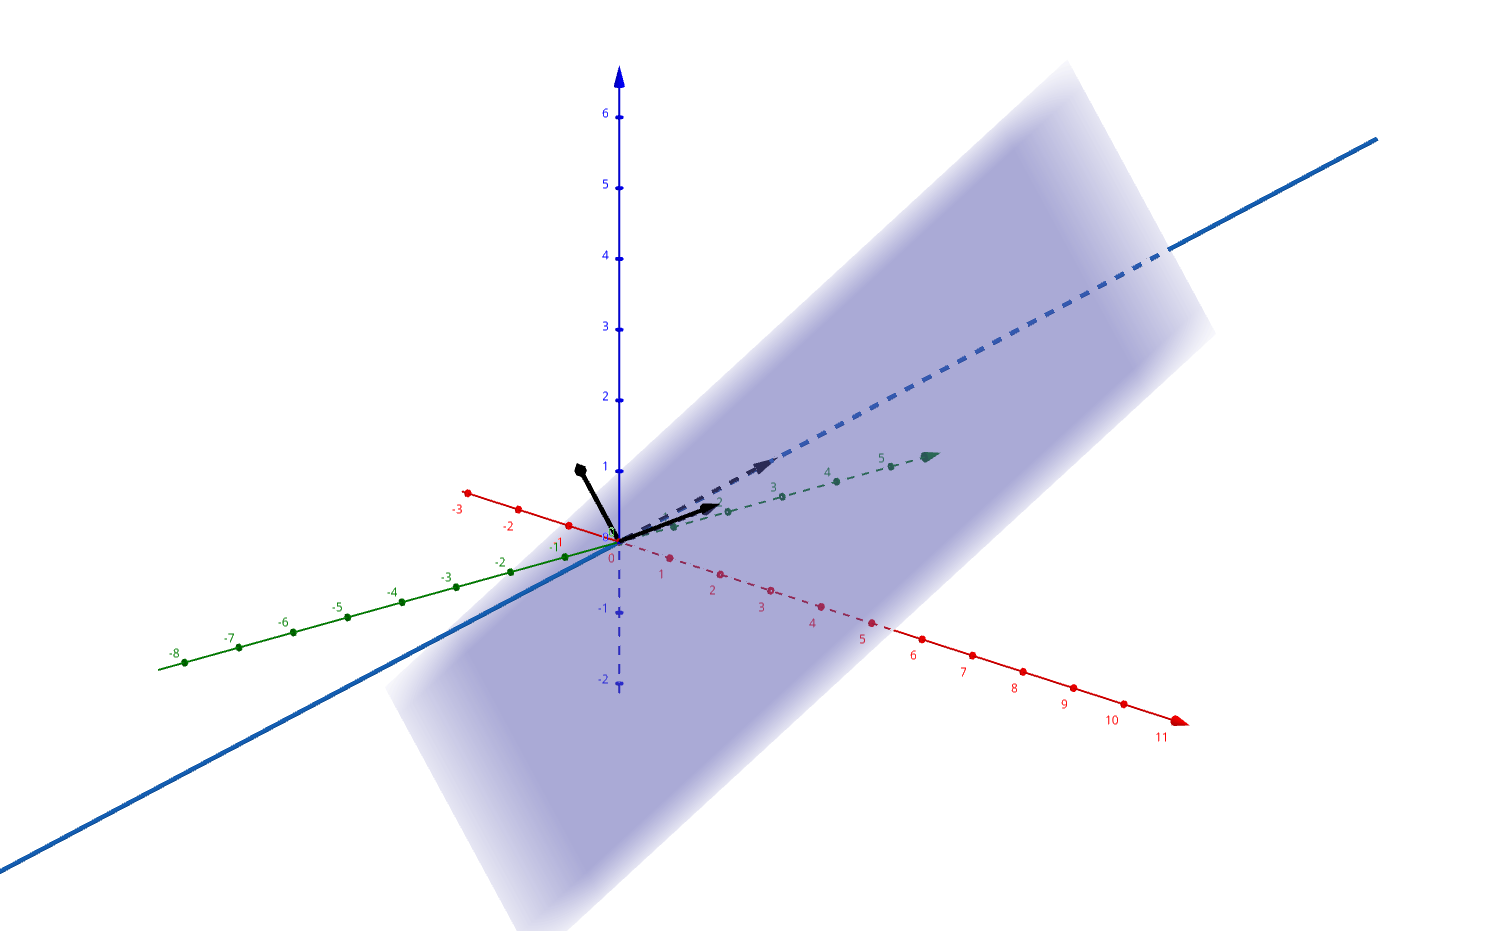
\includegraphics[width=0.95\textwidth]{./img/03-a-1.png}
  \caption{Иллюстрация к задаче № 3 А}
\end{figure}

Составим формулу линейного оператора \(\opA\).

Возьмём вектор с началом в точке \(\coord{0, 0, 0}\)
и произвольными координатами: \(\vec{V} = \coord{x_0, y_0. z_0}\).
Будем искать его проекцию на прямую \(L_1\)
параллельно плоскости \(L_2\).

Сначала найдем уравнение плоскости,
которая проходит через точку \(\coord{x_0, y_0, z_0}\) параллельно \(L_2\).
\(L_2\) задано уравнением \(2x+3y-4z=0\), значит,
вектор нормали имеет координаты: \(\vec{n} = \coord{2, 3, -4}\).
Тогда уравнение плоскости параллельной \(L_2\)
через произвольную точку имеет вид:
\[2(x - x_0) + 3(y - y_0) - 4(z - z_0) = 0\]
Если раскрыть скобки, то получим:
\[2 x + 3 y - 4 z - (2 x_0 + 3 y_0 - 4 z_0) = 0\]
Обозначим \(D = - (2x_0+3y_0-4z_0)\).

Теперь, чтобы найти проекцию точки на прямую \(L_1\) параллельно \(L_2\),
найдем пересечение данной прямой и плоскости проходящей через выбранную
произвольную точку.
Известно, что \(L_1\) определено системой уравнений
\[
  \begin{cases}
    x - y + z = 0 \\
    2x - 3y + 4z = 0
  \end{cases}
\]
Составим систему уравнений, в которую добавим уравнение найденной плоскости.
\begin{align*}
  &\begin{cases}
    x - y + z = 0 \\
    2x - 3y + 4z = 0 \\
    2x + 3y - 4z + D = 0
  \end{cases} \iff
  \begin{cases}
      x - y + z = 0\\
      2x - 3y + 4z = 0\\
      4x + D = 0
  \end{cases} \iff
  \begin{cases}
      x - y + z = 0\\
      2x - 3y + 4z = 0\\
      x = -\frac{D}{4}
  \end{cases} \\
  &\iff
  \begin{cases}
      z = y - x \\
      4z = 3y - 2x \\
      x = -\frac{D}{4}
  \end{cases} \iff
  \begin{cases}
      z = y +\frac{D}{4} \\
      4z = 3y + \frac{D}{2} \\
      x = -\frac{D}{4}
  \end{cases} \iff
  \begin{cases}
      z = y +\frac{D}{4}\\
      4y + D = 3y + \frac{D}{2}\\
      x = -\frac{D}{4}
  \end{cases} \iff
  \begin{cases}
      z = y +\frac{D}{4}\\
      y = -\frac{D}{2}\\
      x = -\frac{D}{4}
  \end{cases} \\
  & \iff
  \begin{cases}
      z = -\frac{D}{4} \\
      y = -\frac{2D}{4} \\
      x = -\frac{D}{4}
  \end{cases} \iff
  \begin{cases}
      z = \frac{1}{4}(2x_0+3y_0-4z_0) \\
      y = \frac{2}{4}(2x_0+3y_0-4z_0) \\
      x = \frac{1}{4}(2x_0+3y_0-4z_0)
  \end{cases}
\end{align*}

Зная координаты точки пересечения, можно составить формулу оператора:\\
\[
  \opA
  \begin{pmatrix}
        x \\ y \\ z
  \end{pmatrix}
  = \frac{1}{4}
  \begin{pmatrix}
        2x + 3y - 4z \\
        4x + 6y - 8z \\
        2x + 3y - 4z
  \end{pmatrix}
\]

Составьте его матрицу в базисе \(\{\vec{i}, \vec{j}, \vec{k}\}\)
пространства \(\mRRR\).

\[
\begin{aligned}
  &\vec{i} = \begin{pmatrix} 1 \\ 0 \\ 0 \end{pmatrix} \qquad
  &\vec{j} = \begin{pmatrix} 0 \\ 1 \\ 0 \end{pmatrix} \qquad
  &\vec{k} = \begin{pmatrix} 0 \\ 0 \\ 1 \end{pmatrix} \\
  &\opA\vec{i} = \frac{1}{4}\begin{pmatrix} 2 \\ 4 \\ 2 \end{pmatrix} \quad
  &\opA\vec{j} = \frac{1}{4}\begin{pmatrix} 3 \\ 6 \\ 3 \end{pmatrix} \quad
  &\opA\vec{k} = \frac{1}{4}\begin{pmatrix} -4 \\ -8 \\ -4 \end{pmatrix}
\end{aligned}
\]

Получившиеся значения образуют столбцы матрицы оператора:
\begin{align*}
  \matA = \frac{1}{4}
  \begin{pmatrix}
    2 & 3 & -4 \\
    4 & 6 & -8 \\
    2 & 3 & -4
  \end{pmatrix}
\end{align*}

Решим задачу о диагонализации полученной матрицы методом спектрального анализа.

Для решения задачи диагонализации матрицы методом спектрального анализа
необходимо найти базис из собственных векторов матрицы,
в котором матрица будет иметь диагональный вид.

Сначала найдем собственные числа оператора.
Для этого решим характеристическое уравнение:
\begin{align*}
    &\det(A - \lambda E) = 0
    \iff
    \begin{vmatrix}
        \frac{1}{2} - \lambda & \frac{3}{4} & -1\\
        1 & \frac{3}{2} - \lambda & -2\\
        \frac{1}{2} & \frac{3}{4} & -1 - \lambda
    \end{vmatrix} = 0 \\
    &
    \left(\frac{1}{2} - \lambda\right)\begin{vmatrix}
        \frac{3}{2} - \lambda & -2\\
        \frac{3}{4} & -1 - \lambda
    \end{vmatrix} - 1 \begin{vmatrix}
        \frac{3}{4} & -1\\
        \frac{3}{4} & -1 - \lambda
    \end{vmatrix} + \frac{1}{2}\begin{vmatrix}
        \frac{3}{4} & -1\\
        \frac{3}{2} - \lambda & -2\\
    \end{vmatrix} = 0 \\
    &
    \left(\frac{1}{2} - \lambda\right)
    \left(
      (\frac{3}{2} - \lambda)(-1 - \lambda)
      - (-2)\cdot\frac{3}{4}\right)
      - 1 \left(\frac{3}{4}(-1-\lambda) - (-1)\cdot \frac{3}{4}\right) + \\
      &+ \frac{1}{2} \left(
        \frac{3}{4}\cdot(-2) - (-1)(\frac{3}{2}-\lambda)
      \right) = 0
    \iff
    \lambda^2(1 - \lambda) = 0
\end{align*}

Получили собственные числа: \(λ_1 = 0, λ_2 = 1\). Теперь найдем
собственные векторы, подставляя \(\lambda_1\) имеем:\\
\begin{align*}
    &\left(
    \begin{matrix}
        \frac{1}{2} & \frac{3}{4} & -1 \\
        1 & \frac{3}{2} & -2 \\
        \frac{1}{2} & \frac{3}{4} & -1
    \end{matrix}
    \right|
    \left. \begin{matrix} 0 \\ 0 \\ 0 \end{matrix} \right)
    \rightsquigarrow
    \left(
    \begin{matrix}
        \frac{1}{2} & \frac{3}{4} & -1 \\
        1 & \frac{3}{2} & -2
    \end{matrix}
    \right|
    \left. \begin{matrix}  0 \\ 0 \end{matrix} \right)
    \rightsquigarrow
    \left(
    \begin{matrix}
        \frac{1}{2} & \frac{3}{4} & -1 \\
        \frac{1}{2} & \frac{3}{4} & -1
    \end{matrix}
    \right|
    \left. \begin{matrix}  0 \\ 0 \end{matrix} \right)
    \rightsquigarrow \\
    &
    \left(
    \begin{matrix} \frac{1}{2} & \frac{3}{4} & -1 \end{matrix}
    \right|
    \left. \begin{matrix}  0  \end{matrix} \right)
    \implies
    \begin{cases}
        x = 2β- \frac{3}{2}α \\
        y = α \\
        z = β
    \end{cases}
\end{align*}

Выберем собственные векторы:
\[
  u_1
  =
  \begin{pmatrix}
    -3 \\ 2 \\ 0
  \end{pmatrix}
  \qquad
  u_2
  =
  \begin{pmatrix}
    2 \\ 0 \\ 1
  \end{pmatrix}
\]

Теперь найдем собственные векторы при \(\lambda_1\):
\begin{align*}
  &
  \left(
  \begin{matrix}
    \frac{1}{2} - 1 & \frac{3}{4} & -1 \\
    1 & \frac{3}{2} - 1 & -2 \\
    \frac{1}{2} & \frac{3}{4} & -1 - 1
  \end{matrix}
  \right|
  \left. \begin{matrix} 0 \\ 0 \\ 0 \end{matrix} \right)
  \rightsquigarrow
  \left(
  \begin{matrix}
    -\frac{1}{2} & \frac{3}{4} & -1 \\
    1 & \frac{1}{2} & -2 \\
    \frac{1}{2} & \frac{3}{4} & -2
  \end{matrix}
  \right|
  \left. \begin{matrix} 0 \\ 0 \\ 0 \end{matrix} \right)
  \rightsquigarrow \\
  &
  \left(
  \begin{matrix}
    -\frac{1}{2} & \frac{3}{4} & -1 \\
    0 & 2 & -4  \\
    0 & \frac{6}{4} & -3
  \end{matrix}
  \right|
  \left. \begin{matrix} 0 \\ 0 \\ 0 \end{matrix} \right)
  \rightsquigarrow
  \left(
  \begin{matrix}
    -\frac{1}{2} & \frac{3}{4} & -1 \\
    0 & 1 & -2 \\
    0 & 6 & -12
  \end{matrix}
  \right|
  \left. \begin{matrix} 0 \\ 0 \\ 0 \end{matrix} \right)
  \rightsquigarrow \\
  &
  \left(
  \begin{matrix}
    -\frac{1}{2} & \frac{3}{4} & -1 \\
    0 & 1 & -2
  \end{matrix}
  \right|
  \left. \begin{matrix} 0 \\ 0 \end{matrix} \right)
  \rightsquigarrow
  \left(
  \begin{matrix}
    -2 & 3 & -4 \\
    0 & 1 & -2
  \end{matrix}
  \right|
  \left. \begin{matrix} 0 \\ 0 \end{matrix} \right) \\
  & \implies
  \begin{cases}
    x = \frac{1}{2}(3y - 4z) = \frac{1}{2}(6α- 4α) = α \\
    y = 2α \\
    z = α
  \end{cases}
\end{align*}

Выберем собственный вектор:
\[
  u_3 = \begin{pmatrix} 1 \\ 2 \\ 1 \end{pmatrix}
\]

Чтобы матрица имела диагональный вид,
нужно выбрать базис образованный ее собственными векторами.
Проверим, что собственные векторы образовывают линейно-независимую систему:
\[
  \begin{pmatrix}
    -3 & 2 & 0 \\
    2 & 0 & 1\\
    1 & 2 & 1
  \end{pmatrix} \rightsquigarrow
  \begin{pmatrix}
    1 & 2 & 1\\
    2 & 0 & 1\\
    -3 & 2 & 0
  \end{pmatrix} \rightsquigarrow
  \begin{pmatrix}
    1 & 2 & 1\\
    0 & -4 & -1\\
    0 & 8 & 3
  \end{pmatrix} \rightsquigarrow
  \begin{pmatrix}
    1 & 2 & 1\\
    0 & -4 & -1\\
    0 & 0 & 1
  \end{pmatrix}
\]
Ранг матрицы, образованной из собственных векторов, равен количеству векторов.
Значит система из собственных образовывает базис.
Составим матрицу перехода из столбцов собственных векторов,
а также обратную матрицу для нее.
\[
  \matP
  =
  \begin{pmatrix}
    -3 & 2 & 1 \\
    2  & 0 & 2 \\
    0  & 1 & 1 \\
  \end{pmatrix} ,\qquad
  {\matP}^{-1}
  =
  \begin{pmatrix}
    -\frac{1}{2} & -\frac{1}{4} & 1 \\
    -\frac{1}{2} & -\frac{3}{4} & 2 \\
    \frac{1}{2} & \frac{3}{4} & -1
  \end{pmatrix}
\]

Воспользуемся формулой \(\matA_D = {\matP}^{-1} \matA \matP\)
\begin{align*}
  \matA_D
  &=
  \begin{pmatrix}
    -\frac{1}{2} & -\frac{1}{4} & 1 \\
    -\frac{1}{2} & -\frac{3}{4} & 2 \\
    \frac{1}{2} & \frac{3}{4} & -1
  \end{pmatrix}
  \begin{pmatrix}
    \frac{1}{2} & \frac{3}{4} & -1 \\
    1 & \frac{3}{2} & -2 \\
    \frac{1}{2} & \frac{3}{4} & -1
  \end{pmatrix}
  \begin{pmatrix}
      -3 & 2 & 1 \\
      2  & 0 & 2 \\
      0  & 1 & 1 \\
  \end{pmatrix} \\
  \matA_D
  &=
  \begin{pmatrix}
    0 & 0 & 0\\
    0 & 0 & 0\\
    \frac{1}{2} & \frac{3}{4} & -1
  \end{pmatrix}
  \begin{pmatrix}
      -3 & 2 & 1 \\
      2  & 0 & 2 \\
      0  & 1 & 1 \\
  \end{pmatrix} \\
  \matA_D
  &=
  \begin{pmatrix}
        0 & 0 & 0\\
        0 & 0 & 0\\
        0 & 0 & 1
  \end{pmatrix}
\end{align*}


На построенном ранее графике изобразим базис,
в котором матрица линейного оператора \(\opA\) имеет диагональный вид.
\begin{figure}[!htbp]
  \centering
  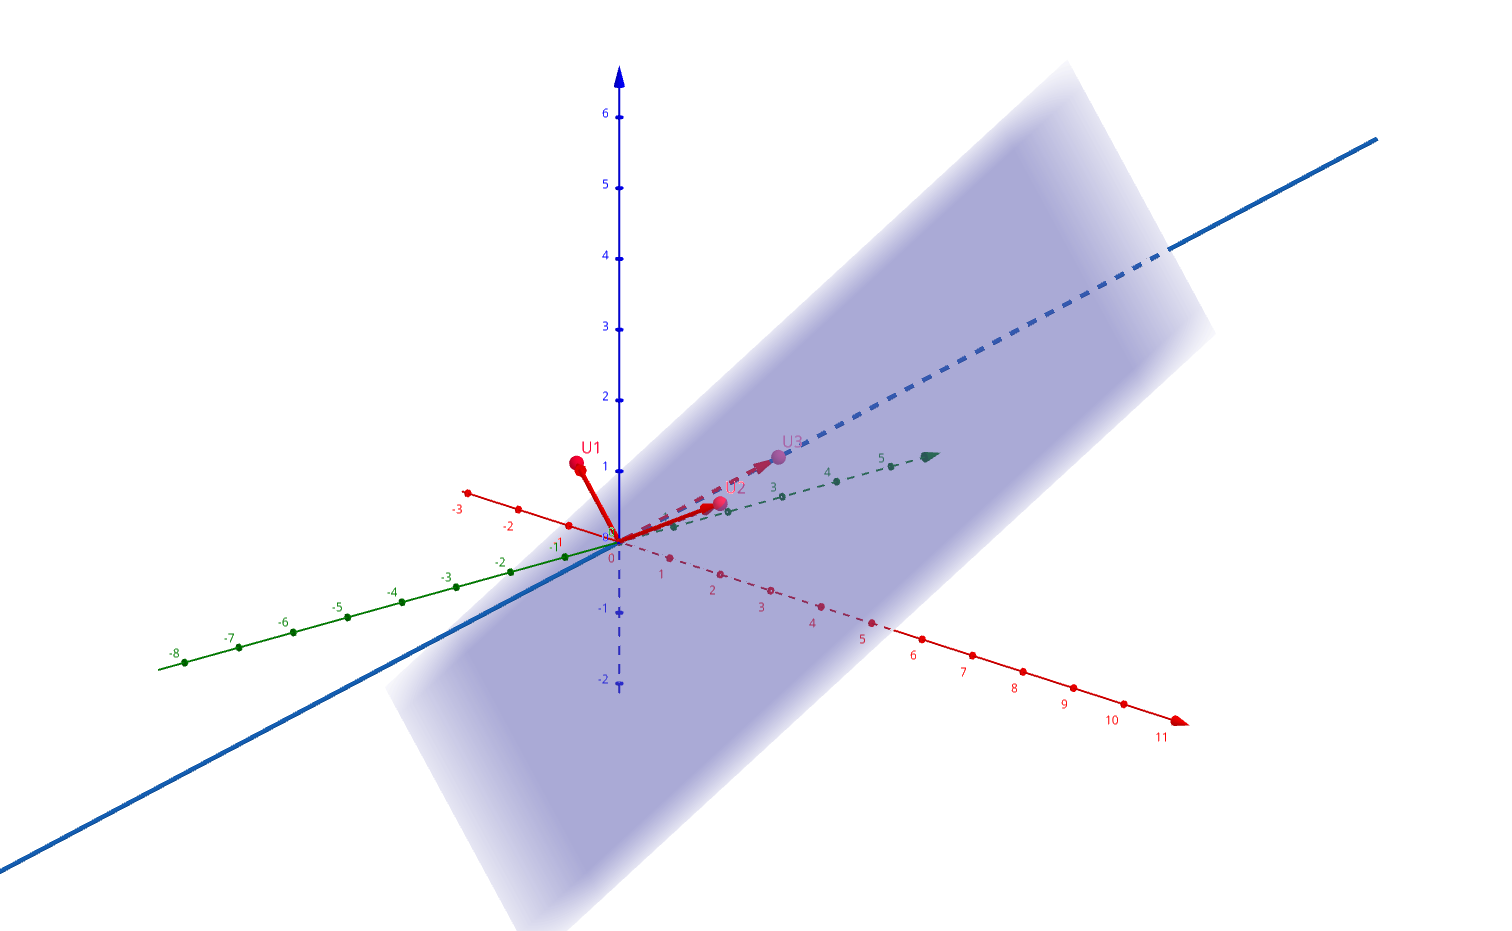
\includegraphics[width=0.95\textwidth]{./img/03-a-2.png}
  \caption{Иллюстрация к задаче № 3 А. \protect\footnotemark}
\end{figure}

\footnotetext{
  \href{https://www.geogebra.org/calculator/gbkddqnm}{Ссылка на Geogebra}
}

Базис, в котором матрица линейного оператора имеет диагональный вид,
состоит из собственных векторов этого оператора.
В этом базисе можно упростить вычисления значения линейного оператора,
так как матрица оператора в нем диагонализирована.
